
\section{IMPLEMENTATION OF THE NON-LINEAR FORECASTING TECHNIQUE}

The technique presented in this thesis was implemented in the Anaconda distribution of Python 2.7. Array manipulation was implemented in Numpy \cite{numpy}. Plotting was handled by Matplotlib \cite{matplotlib} and stylized by Seaborn \cite{seaborn}. The heart of the non-linear forecasting technique is the near neighbor algorithm from Sci-kit Learn \cite{scikit}. The work was completed in IPython Notebooks \cite{ipython}. The raw code for this project and accompanying IPython Notebooks can be found at nickc1.github.com.

The following subsections will go into more detail about the non-linear forecasting technique, but the general algorithm follows these steps:

\begin{enumerate}
\item Input one-dimensional time series or two-dimensional image.
\item Calculate the lag value which is the first minimum of the mutual information.
\item Split data into training set and testing set.
\item Embed each in an m-dimensional space.
\item Calculate the distance from all vectors in the test set to all vectors in the training set.
\item Average the evolution of the K closest vectors in the training set to make forecasts for the testing set.
\item Compare forecasts to actual evolution of the system.
\item Repeat steps 6 and 7 with K ranging from 1 to 25\% of the total size of the training set.
\item Repeat steps 4 through 8 to find the embedding dimension with highest forecast skill.
\item Calculate the Deterministic Metric.
\end{enumerate}
%=================================================

\subsection{LAG VALUE CALCULATION}
Before embedding a time series or an image, a lag value must be calculated. Lag values are given by the first minimum in the mutual information. A calculation of the mutual information for a time series, $X$, is implemented in python as:

\lstinputlisting[language=Python]{code_samples/mutual_information.py}

In this implementation, $X$ is the time series and $max\_lag$ is the maximum number of time steps that the time series is shifted. After shifting the time series and binning the time series values, sci-kit learn's mutual information implementation is calculated as,

$$MI(U,V) = \sum_{i=1}^R \sum_{j=1}^C P(i,j) log\frac{P(i,j)}{P(i)P'(j)}.$$

Here $P(i)$ is the probability of a random sample occurring in $U_i$ (the un-shifted time series) and $P'(j)$ is the probability of a random sample occurring in $V_j$ (the shifted time series). $P(i,j)$ is the probability of both $U_i$ and $V_j$ occurring in the same random sample. This function will output a series of mutual information values corresponding to the amount that the time series is shifted. For more information on lagged values for reconstructing state spaces refer to Reference \cite{mutual_info}.

For two-dimensional images, the mutual information along each row and each column is calculated and then summed together. This is implemented in python as,

\lstinputlisting[language=Python]{code_samples/spatial_mutual_info.py}

In this implementation $M$ is the input image, $max\_lag$ is the maximum amount of image shift, and $percent\_calc$ is the percent of rows and columns that are summed over to calculate the mutual information. The $percent\_calc$ is used to speed up the computation. Experimentation has shown that no accuracy is lost summing over a smaller amount of the rows or columns for the mutual information calculation. This function utilizes the one dimensional $mutual\_information$ function above.

%===========================================[Splitting into test and train set]
\subsection{TRAINING AND TESTING SETS}

When implementing the non-linear forecasting technique, the time series and images are split into a training set and a testing set. Usually, the training set consists of the first two-thirds of the data and the testing set is composed of the final one-third. By splitting the time series and images, forecasts for the test set using the training set can be compared to the actual values of the testing set. The accuracy of the forecasts can then be quantified. An implementation in python is given as,

\lstinputlisting[language=Python]{code_samples/2d_split.py}

This function is capable of handling both one dimensional and two dimensional inputs. The function utilizes the $try$, $except$ block to determine if the input is one dimensional or two dimensional.

%==========================================[Embedding]
\subsection{EMBEDDING}
The testing set and training sets are embedded independently in an m-dimensional space. The dimensionality, $m$, is iterated at a later step using a false near neighbors technique to determine the optimal embedding \cite{nonlinear_book}. An example of a single embedded vector of dimension 3 and a lag value of 2 for the first eight values of a time series, $T$ is given by the green squares in Figure \ref{1d_embedding}. 

\begin{figure}[htbp] %  figure placement: here, top, bottom, or page
   \centering
   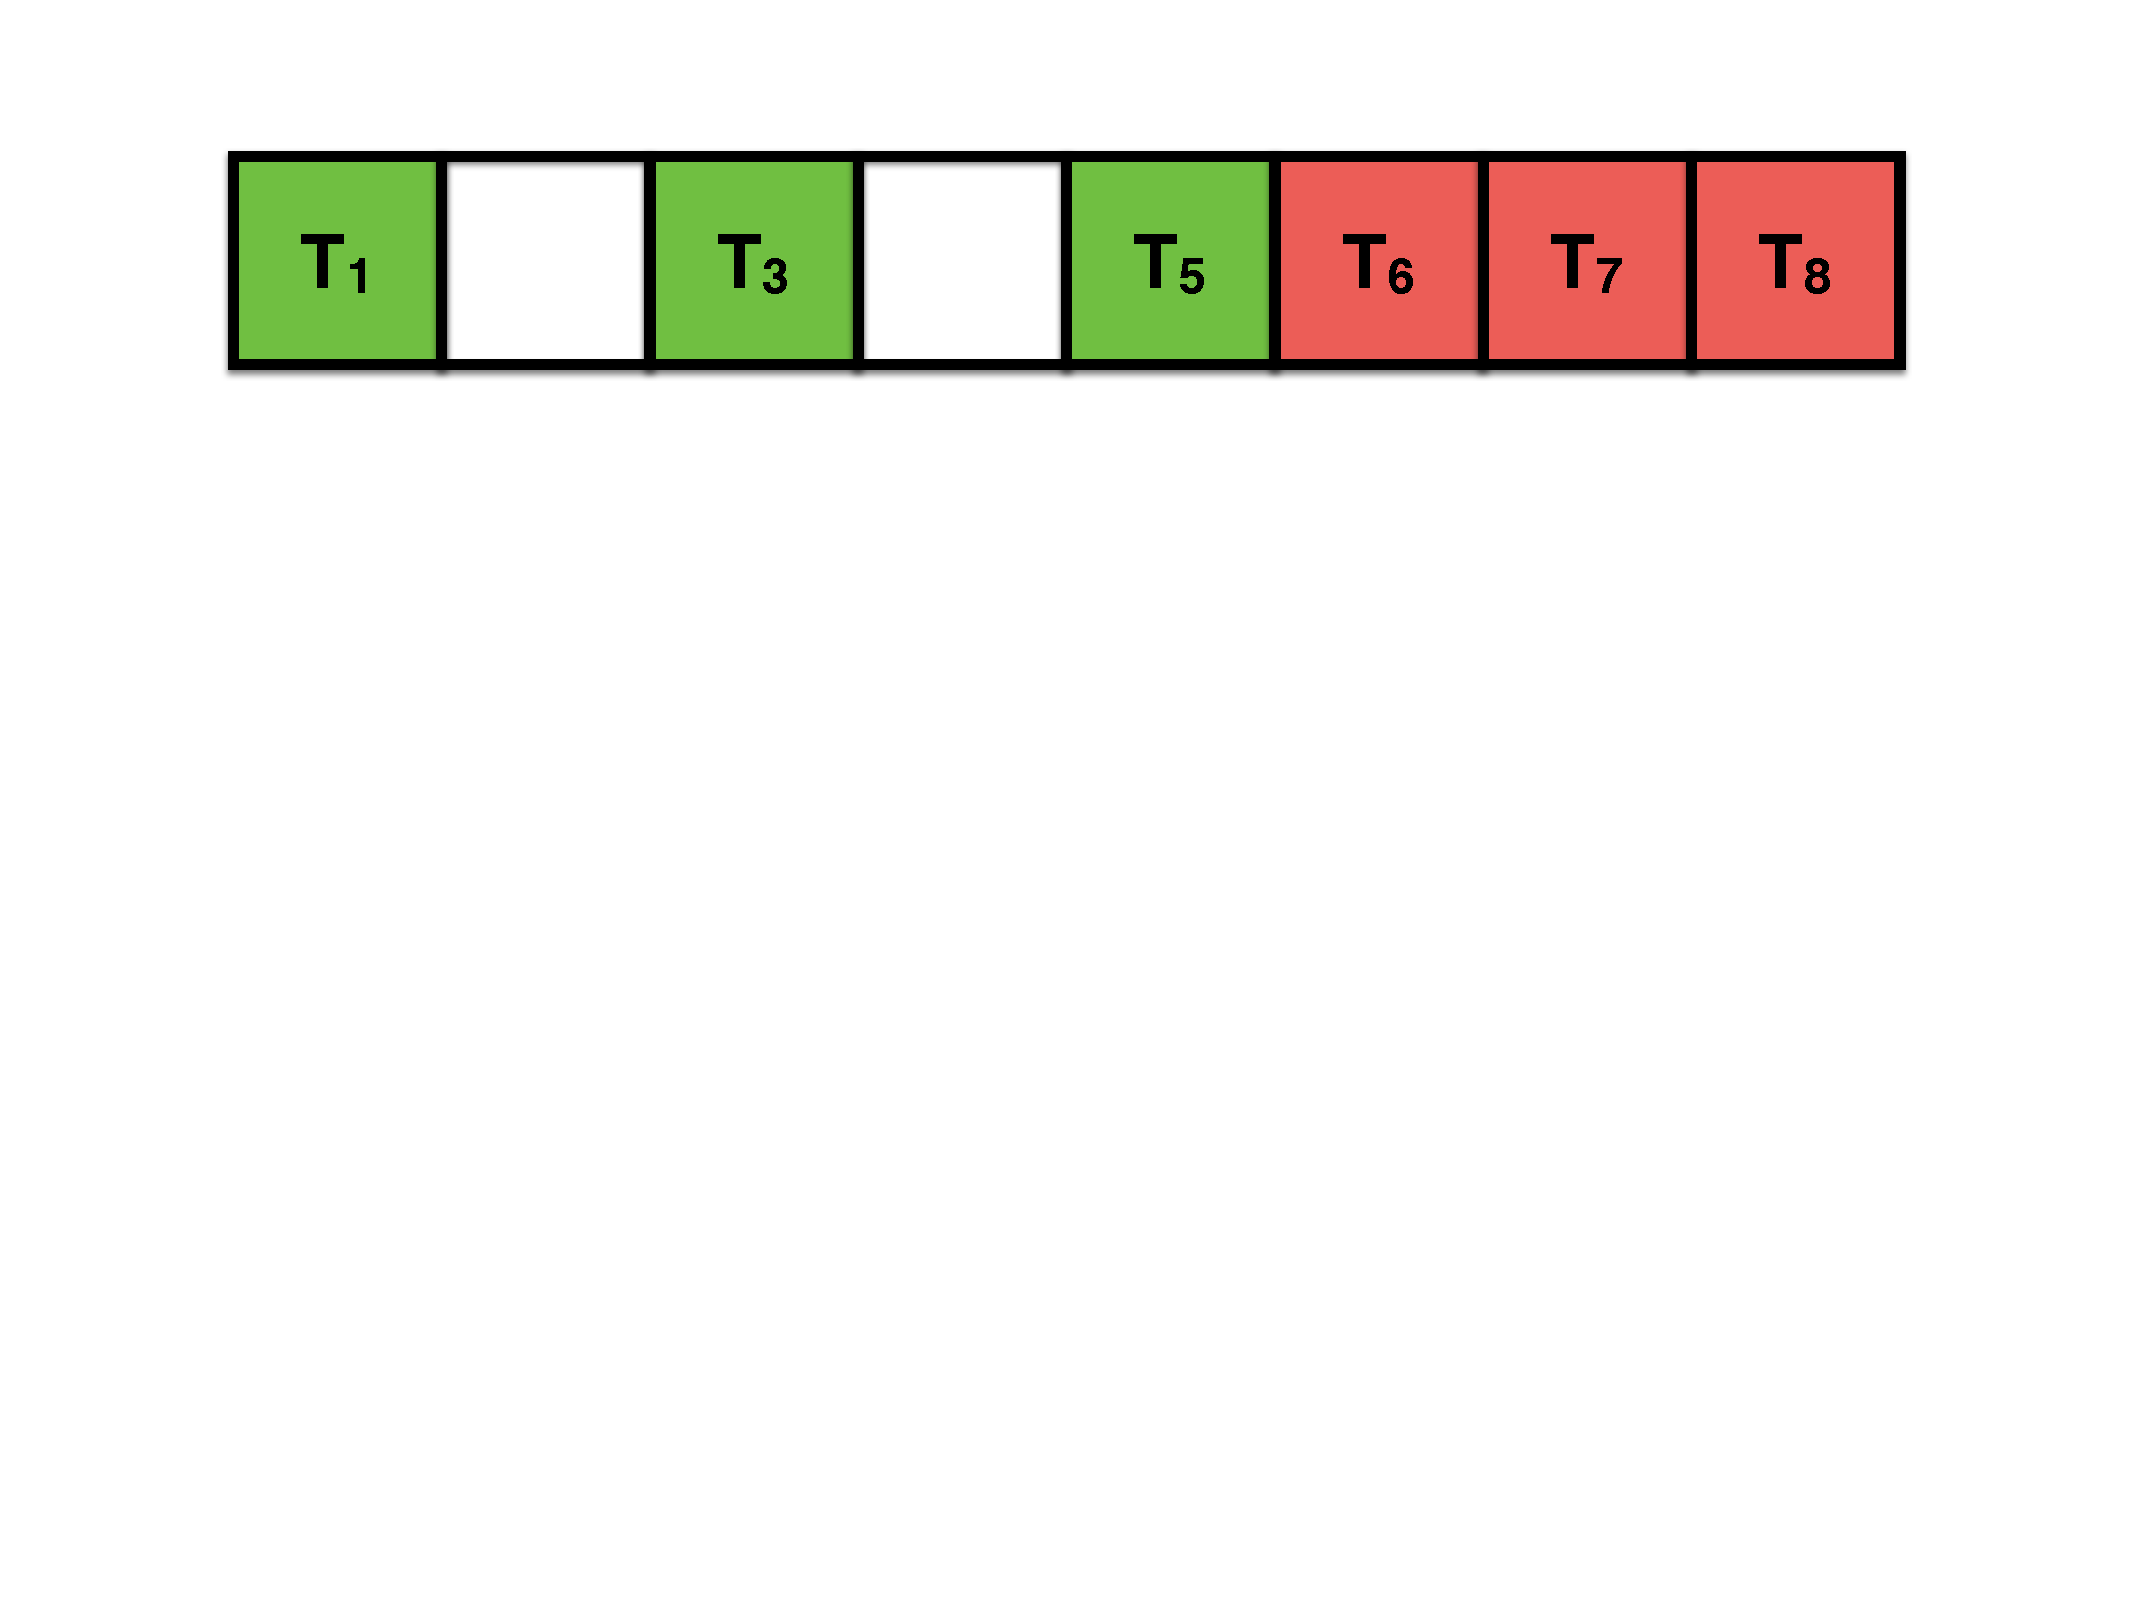
\includegraphics[width=3in]{code/1d_reshape.pdf} 
   \caption{Embedding technique illustrating an embedding dimension of three with lag value of two. Green is the embedded time series values and red is the forecast y values.}
   \label{1d_embedding}
\end{figure}

The green squares are shifted by one to embed the next vector in the $m$-dimensional space. All of the embedded vectors are stored in a matrix, $X$. The red squares in Figure \ref{1d_embedding} represent the evolution vectors of the system. Likewise, the red squares are shifted over and the next evolution vector is obtained. These values are stored in a matrix $y$. The process is repeated for the embedded vectors and evolution vectors over the length of the time series. A generalization of this technique is given by:

\[
X=
\begin{bmatrix}
    T_{t} & T_{t+\tau} & T_{t+2\tau} & \dots  & T_{t+m\tau} \\
    T_{t+1} & T_{t+1 + \tau} & T_{t+1 + 2\tau} & \dots  & T_{t+1 +m\tau} \\
    \vdots & \vdots & \vdots & \ddots & \vdots \\
    T_{t+n} & T_{t+n+\tau} & T_{t+n + 2\tau} & \dots  & T_{t+ n+  m\tau}
\end{bmatrix}
\]

\[
Y=
\begin{bmatrix}
    T_{t+m\tau + 1} & T_{t+m\tau + 2}  & \dots  & T_{t+m\tau + p} \\
    T_{t+1 + m\tau + 1} & T_{t+1 + m\tau + 2}  & \dots  & T_{t+1 + m\tau + p} \\
    \vdots & \vdots & \vdots & \ddots & \vdots \\
    T_{t+n + m\tau + 1} & T_{t+n + \tau + 2}  & \dots  & T_{t+n +m\tau + p}
\end{bmatrix}
\]

Where $\tau$ is the lag value, $m$ is the embedding dimension, $p$ is the forecast distance, and $n$ is the length of $T$ minus the prediction distance. This implemented in python is given as,

\lstinputlisting[language=Python]{code_samples/lag_reshape.py}

The two-dimensional version of the embedding is similar to the time series version. An example embedding of a spatio-temporal image is given in Figure \ref{2d_embedding}. 

\begin{figure}[htbp] %  figure placement: here, top, bottom, or page
   \centering
   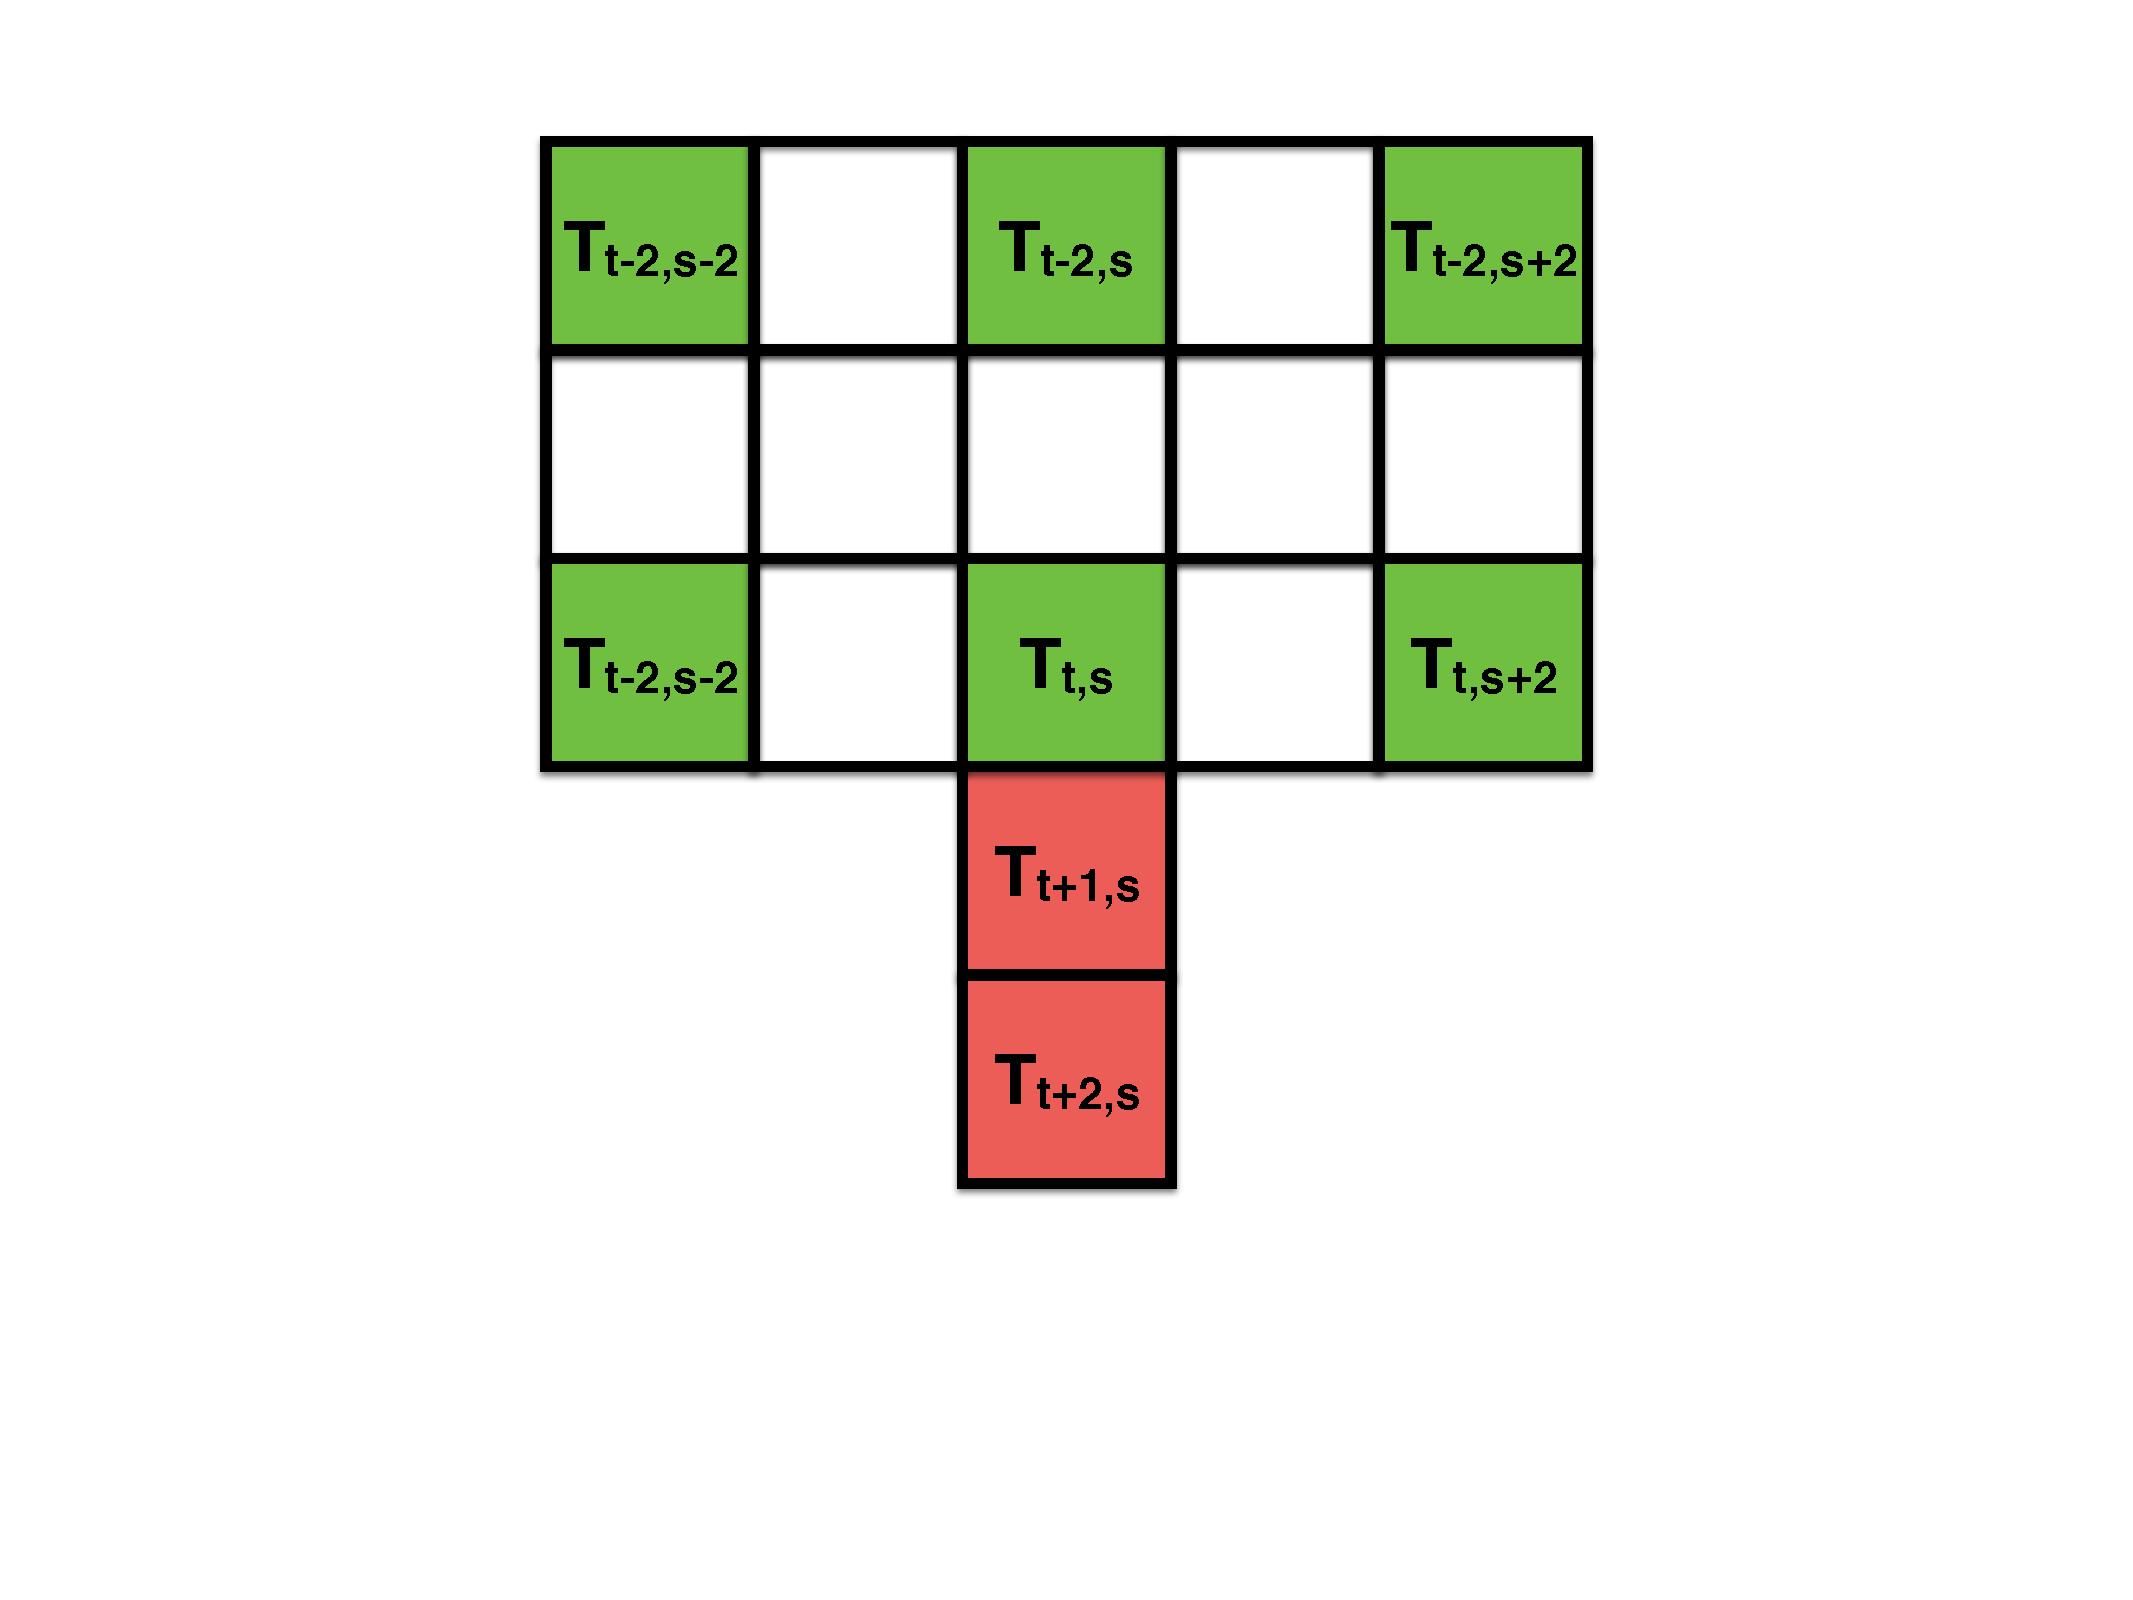
\includegraphics[width=3in]{code/2d_reshape.pdf} 
   \caption{Embedding technique illustrating an embedding dimension of six with lag value of two in both space and time. Green is the embedded spatio-temporal series values and red is the forecast y values.}
   \label{2d_embedding}
\end{figure}


The embedded vector (green) is six dimensional and has a spatial lag of 2 and a temporal lag of 2. The evolution vector is given in red. Both the embedded vector and the evolution vector are shifted over and the next embedded vector and evolution vector are calculated. The embedded vectors are stored in a matrix, $\vec X$, and the evolution vectors are stored in a matrix, $y$. Formally, $\vec X$ and $\vec Y$ can be defined as,

$$\vec X_{(t,s)}(x) = (x_{(t,s)}, x_{(t-\tau,s)}, \dots, x_{t-(m-1)\tau,s\pm \frac{n-1}{2}\sigma}),$$

$$\vec Y_{(t,s)}(x) = (x_{(t+1,s)}, x_{(t+2,s)}, \dots, x_{(t+p,s)}   ),$$

where $x$ is the spatio-temporal image, $s$ refers to the spatial component of the series, $\tau$ is the spatial lag, $\sigma$ is the spatial embedding dimension, and $p$ is the forecast distance. An implementation in python is given by:

\lstinputlisting[language=Python]{code_samples/ft_reshape.py}

This implementation allows for a certain percent of the space to be transformed into embedded vectors and evolution vectors. This is for computational efficiency in the calculation of distances. Furthermore, experimentation has shown that it is not necessary to test every single location. For most systems 25\% is effective. Additionally note that the lag values and embedding dimension are set up to be tuples. The first value is the lag or embedding dimension down the rows and the second value is across the columns. 


%=====================================================[KNN]
\subsection{K-NEAREST NEIGHBOR ALGORITHM}

At the heart of the non-linear forecasting technique is the K-Nearest Neighbors Algorithm \cite{nearest_neighbor}. The algorithm calculates the euclidean distances from each of the testing embedded vectors, $\vec X_{test}$ to each of the training embedded vectors, $\vec X_{train}$. The distance from the $i'th$ embedded train vector to the $j'th$ embedded test vector is,

$$ d_i( X_{train,i}, X_{test,j} ) = \sqrt{ (X_{train,i}-X_{test,j})^2}$$


The $y_{train}$ values of the closest $k$ vectors in the training set are averaged and a forecast, $y_p$, is made. This takes the form,

$$ y_{p} = \frac{ y_{train,1} + y_{train,2} + \dots  y_{train,k} } {k}. $$


The results of the forecast is then compared to the actual evolution vectors and the coefficient of determination, $R^2$ is calculated as,

$$R^2 = 1 - \frac{ \sum(y_i - f_i)^2 }  {\sum(y_i - \bar y )^2},$$

where $y_i$ is the $i^{th}$ prediction, $f_i$ is the true value, and $\bar y$ is the mean of the $y$ values. The near neighbor algorithm is implemented in python as,


\lstinputlisting[language=Python]{code_samples/nn_check.py}

This function utilizes sci-kit learn's $kneighbors$ function for efficient calculation of the distances from the testing set to the training set. It also has the ability to calculate weighted averages. For this paper, uniform weightings are used throughout.

In order to forecast discrete classes, the implementation is the same except the hamming distance is used to calculate the proximity of points and the mode of the $k$ nearest $y\_train$ class labels is the forecast where the mode is calculated as,

$$ Y_{p} = mode(y_{1}, y_{2}, \dots,  y_k). $$

This slightly different version is implemented in python as,

\lstinputlisting[language=Python]{code_samples/nnclassification.py}



Finally in order to evaluate the forecasts a metric is developed that calculates the percent correctly predicted. This is represented simply as,
$$ P = \frac{ N_c} {N_t}, $$
where $N_c$ is the number correctly predicted and $N_t$ is the total number of predictions. The algorithm is then iterated over a number of embedding dimensions $m$ to find the value of $m$ that gives the highest forecast skill. This is implemented in python as,


\lstinputlisting[language=Python]{code_samples/class_compare.py}

%===================================================== [Deterministic Metric]
\subsection{DETERMINISTIC METRIC}

The deterministic metric attempts to quantify the amount of determinism in a given time series or image. After finding the best embedding dimension, $m$, the algorithm is calculated as,

$$ D = \sum^n_{d=1} max(R^2_{d,\%K<12.5}) - min(R^2_{d,\%K\geq12.5}). $$

This function is implemented in python as,

\lstinputlisting[language=Python]{code_samples/deterministic_metric.py}



%====================================================[Example: One Dimensional]
\subsection{EXAMPLE: ONE-DIMENSIONAL}

Here the the $x$ values from the lorenz system are used to illustrate the workflow for the non-linear forecasting technique. The first step is to generate the time series and import the needed libraries. This is done as python as,

\lstinputlisting[language=Python]{code_samples/1d_example_lorenz_ts.py}

The required libraries are imported and Seaborn is used to style the plots. Scipy's integrate function is used to integrate the lorenz equations. The resulting plot is shown in Figure \ref{create_series}.

\begin{figure}[htbp] %  figure placement: here, top, bottom, or page
   \centering
   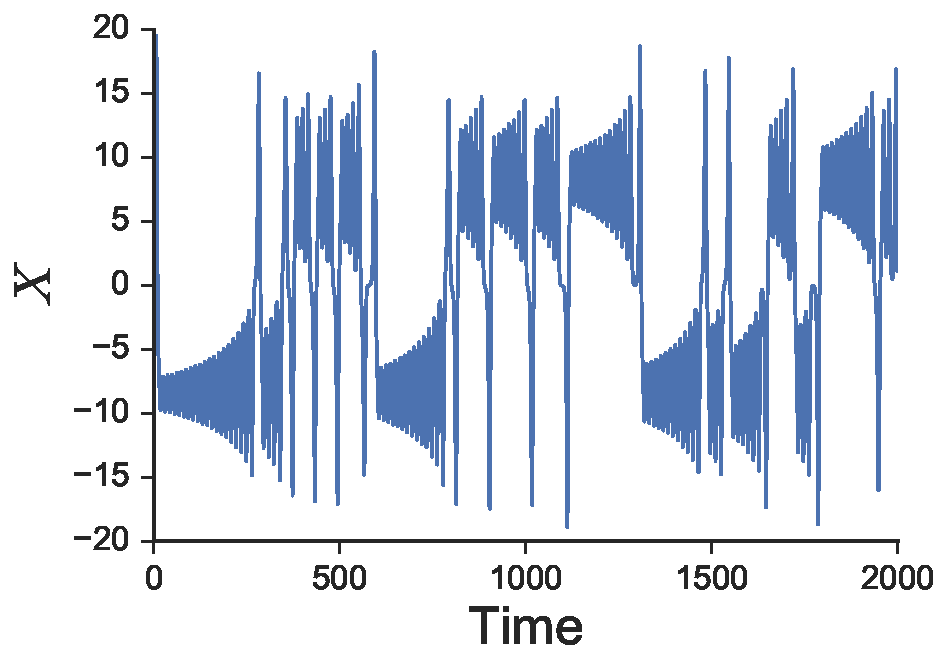
\includegraphics[width=3in]{code/lorenz_ts.pdf} 
   \caption{$X$ values from the lorenz equations.}
   \label{create_series}
\end{figure}


The next step is to calculate a lag value for the system. This is done by finding the first minimum of the mutual information between a shifted time series and an unshifted one. The results of the code are shown in Figure \ref{code_mutual_info}.

\lstinputlisting[language=Python]{code_samples/1d_example_mutual_info.py}

\begin{figure}[htbp] %  figure placement: here, top, bottom, or page
   \centering
   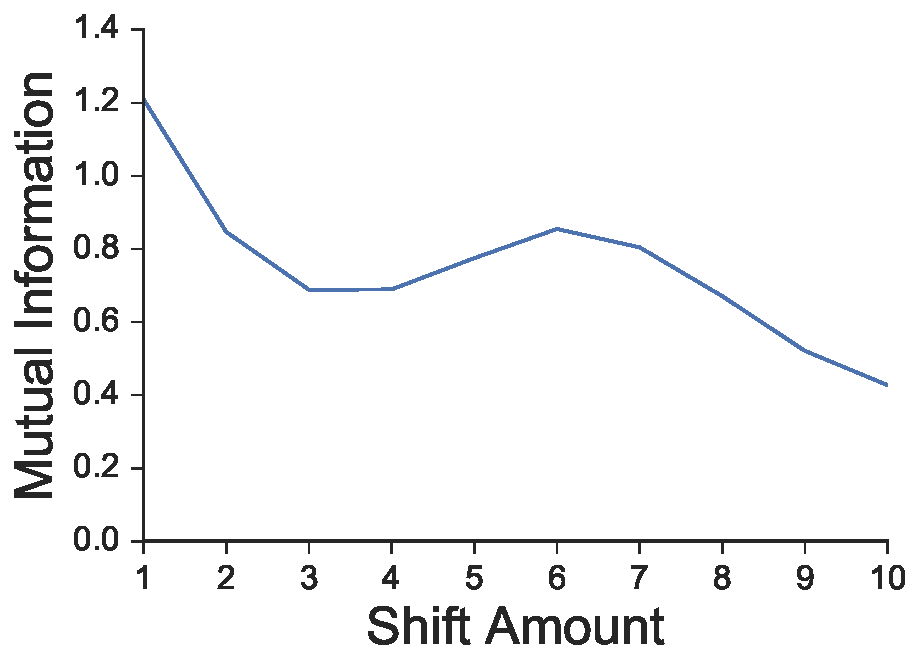
\includegraphics[width=3in]{code/lorenz_mutual_info.pdf} 
   \caption{Mutual information between the shifted $X$ values and unshifted $X$ values from the lorenz equations.}
   \label{code_mutual_info}
\end{figure}

Now we can split our time series into a testing set and a training set. This is done in python as,

\lstinputlisting[language=Python]{code_samples/1d_example_split.py}


The next step is to iterate over the embedding dimension $m$ to find the embedding that provides the maximum forecast skill. This takes three functions: $nnEfficient$, $score$, and $em\_check$. $em\_check$ iterates through $m$ to find the ideal embedding, while $nnEfficient$ finds the near neighbors in the reconstructed state space. $score$ quantifies the forecast skill. The results are shown in Figure \ref{best_embedding}

\lstinputlisting[language=Python]{code_samples/1d_example_find_embedding.py}

\begin{figure}[htbp] %  figure placement: here, top, bottom, or page
   \centering
   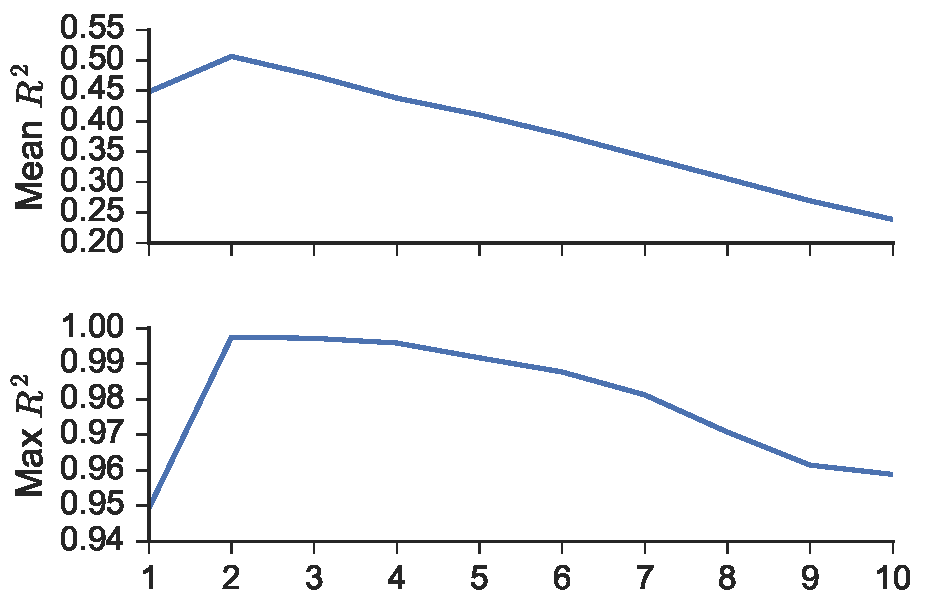
\includegraphics[width=3in]{code/lorenz_best_em.pdf} 
   \caption{Coefficient of determination $R^2$ versus embedding dimension, $m$.}
   \label{best_embedding}
\end{figure}

According to the ideal embedding for the time series is two. This is then used to embed our data. We can visualize the embedding through the code below that produces Figure \ref{code_embedding}.


\lstinputlisting[language=Python]{code_samples/1d_example_embedded_lorenz.py}

\begin{figure}[htbp] %  figure placement: here, top, bottom, or page
   \centering
   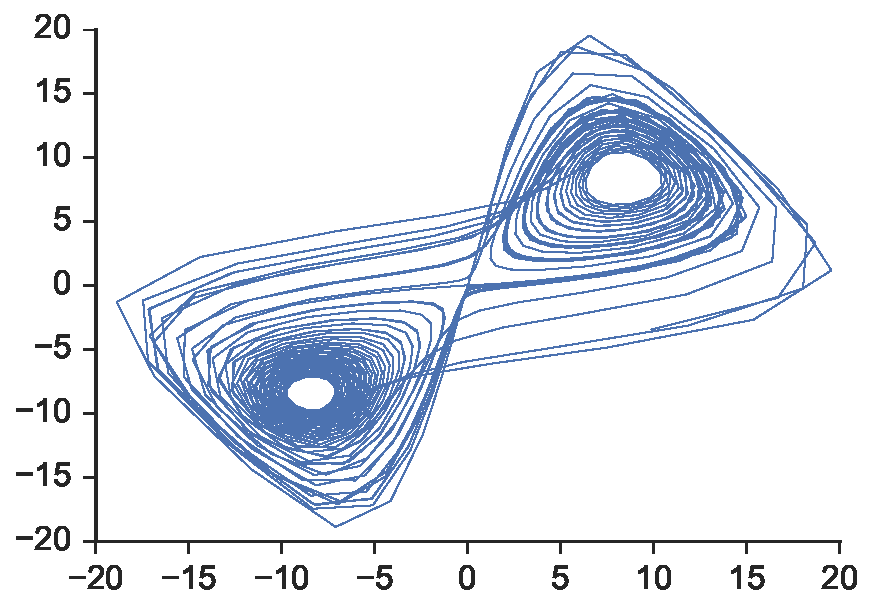
\includegraphics[width=3in]{code/lorenz_embedded.pdf} 
   \caption{Two-dimensional embedding of the lorenz $X$ values.}
   \label{code_embedding}
\end{figure}



Finally we can run $nnEfficient$ and produce a contour plot of the results in order to visualize the trends in forecast skill with respect to the number of neighbors used. The code below produces Figure \ref{code_contour}


\lstinputlisting[language=Python]{code_samples/1d_example_final_step.py}

\begin{figure}[htbp] %  figure placement: here, top, bottom, or page
   \centering
   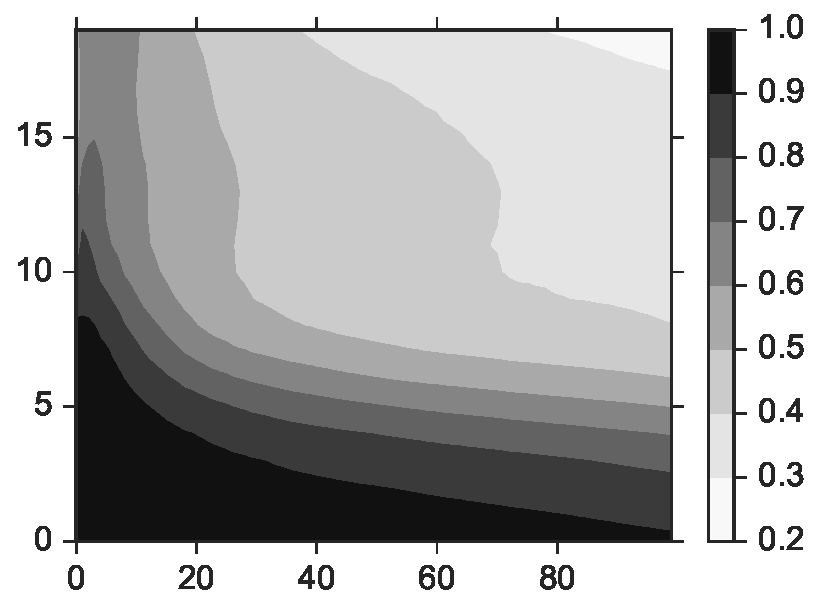
\includegraphics[width=3in]{code/lorenz_contour.pdf} 
   \caption{Coefficient of determination $R^2$ versus embedding dimension, $m$.}
   \label{code_contour}
\end{figure}









% $$X = y$$

% where, 
% \[
% X=
% \begin{bmatrix}
%     x_{11} & x_{12} & x_{13} & \dots  & x_{1n} \\
%     x_{21} & x_{22} & x_{23} & \dots  & x_{2n} \\
%     \vdots & \vdots & \vdots & \ddots & \vdots \\
%     x_{d1} & x_{d2} & x_{d3} & \dots  & x_{dn}
% \end{bmatrix}
% \]

% \[
% y=
% \begin{bmatrix}
%     y_{11} & y_{12} & y_{13} & \dots  & y_{1n} \\
%     y_{21} & y_{22} & y_{23} & \dots  & y_{2n} \\
%     \vdots & \vdots & \vdots & \ddots & \vdots \\
%     y_{d1} & y_{d2} & y_{d3} & \dots  & y_{dn}
% \end{bmatrix}
% \]

% $X$ is referred to as the features (the variables that are used to predict $y$) and $y$ is referred to as the target variables. Each sample, $d$, has dimensionality $n$. This is to say, $(x_{d1}, x_{d2}, x_{d3}, \dots, x_{dn})$ is used to predict $(y_{d1}, y_{d2}, y_{d3}, \dots, y_{dn})$.




% In order to make predictions about a single sample in the testing set, the euclidean distance from the feature vectors in the testing set to the feature vectors in the training set are calculated as:

% $$ d( (x_{rd1},x_{rd2}, \dots, x_{rdn}) , (x_{td1},x_{td2}, \dots, x_{tdn}) ) =$$
% $$ \sqrt{ (x_{rd1}-x_{td1})^2 + (x_{rd2}-x_{td2})^2 + \dots + (x_{rdn}-x_{tdn})^2  }$$

% The $y_r$ values of the closest $k$ vectors in the training set are averaged together to make a prediction, $Y_p$ about the testing set. This takes the form,

% $$ Y_{p} = \frac{ y_{1} + y_{2} + \dots  y_k } {k}. $$

% If the prediction is a discrete class label, then the mode is taken. This takes the form,

% $$ Y_{p} = mode(y_{1}, y_{2}, \dots,  y_k) $$

% After predicting all of the samples appropriately, the next step is to make some measurement about the accuracy of the predictions. For regression problems, the coefficient of determination is calculated as,

% $$R^2 = 1 - \frac{ \sum(y_i - f_i)^2 }  {\sum(y_i - \bar y )^2}$$

% Where $y_i$ is the $i$ prediction, $f_i$ is the true value, and $\bar y$ is the mean of the $y$ values. 

% For classification problems, the percent correctly predicted is calculated as, 

% $$ P = \frac{ N_c} {N_t}, $$

% where $N_c$ is the number correctly predicted and $N_t$ is the total number of predictions.


% %===================================================[One Dimensional Regression]
% \subsection{One Dimensional Regression}

% To apply the near neighbor algorithm to a time series, first the time series must be embedded in order to apply the algorithm. Given a time series $T$, it is reshaped to produce a set of feature vectors $X$ and a set of target vectors $y$ and take the form of,

% \[
% X=
% \begin{bmatrix}
%     T_{t} & T_{t+\tau} & T_{t+2\tau} & \dots  & T_{t+m\tau} \\
%     T_{t+1} & T_{t+1 + \tau} & T_{t+1 + 2\tau} & \dots  & T_{t+1 +m\tau} \\
%     \vdots & \vdots & \vdots & \ddots & \vdots \\
%     T_{t+n} & T_{t+n+\tau} & T_{t+n + 2\tau} & \dots  & T_{t+ n+  m\tau}
% \end{bmatrix}
% \]

% \[
% Y=
% \begin{bmatrix}
%     T_{t+m\tau + 1} & T_{t+m\tau + 2}  & \dots  & T_{t+m\tau + p} \\
%     T_{t+1 + m\tau + 1} & T_{t+1 + m\tau + 2}  & \dots  & T_{t+1 + m\tau + p} \\
%     \vdots & \vdots & \vdots & \ddots & \vdots \\
%     T_{t+n + m\tau + 1} & T_{t+n + \tau + 2}  & \dots  & T_{t+n +m\tau + p}
% \end{bmatrix}
% \]

% where $\tau$ is the lag value, $m$ is the embedding dimension, $p$ is the forecast distance, and $n$ is the length of $T$ minus the prediction distance. 

% After reshaping the time series into feature vectors, $X$, and a target vectors, $y$, the vectors must be split into a traing set and a testing set. A python implementation is given by,

% \newpage
% \lstinputlisting[language=Python]{code_samples/train_test_split.py}

% Next, the reshaped training set and testing set can be fed into a near neighbor algorithm. Here, an implementation in Sci-kit Learn is used.

% \newpage
% \lstinputlisting[language=Python]{code_samples/nn_check.py}

% All the pieces have been coded, now everything is given one wrapper function so that a time series can be given and out pops the analysis over a range of near neighbors.


% \newpage
% \lstinputlisting[language=Python]{code_samples/train_predict.py}




% %====================================================[Two-Dimensional Regression]
% \subsection{Two-Dimensional Regression}

% Now to extend the algorithm to two dimensions, all that needs to be done is to alter the reshaping technique. Other than that, everything is the same. Feature vectors in the spatial sense are represented as: 

% $$y_{(t,s)}(x) = (x_{t,s)}, x_{(t-\tau,s)}, \dots, x_{t-(m-1)\tau,s\pm \frac{n-1}{2}\sigma})$$

% \begin{figure}[htbp] %  figure placement: here, top, bottom, or page
%    \centering
%    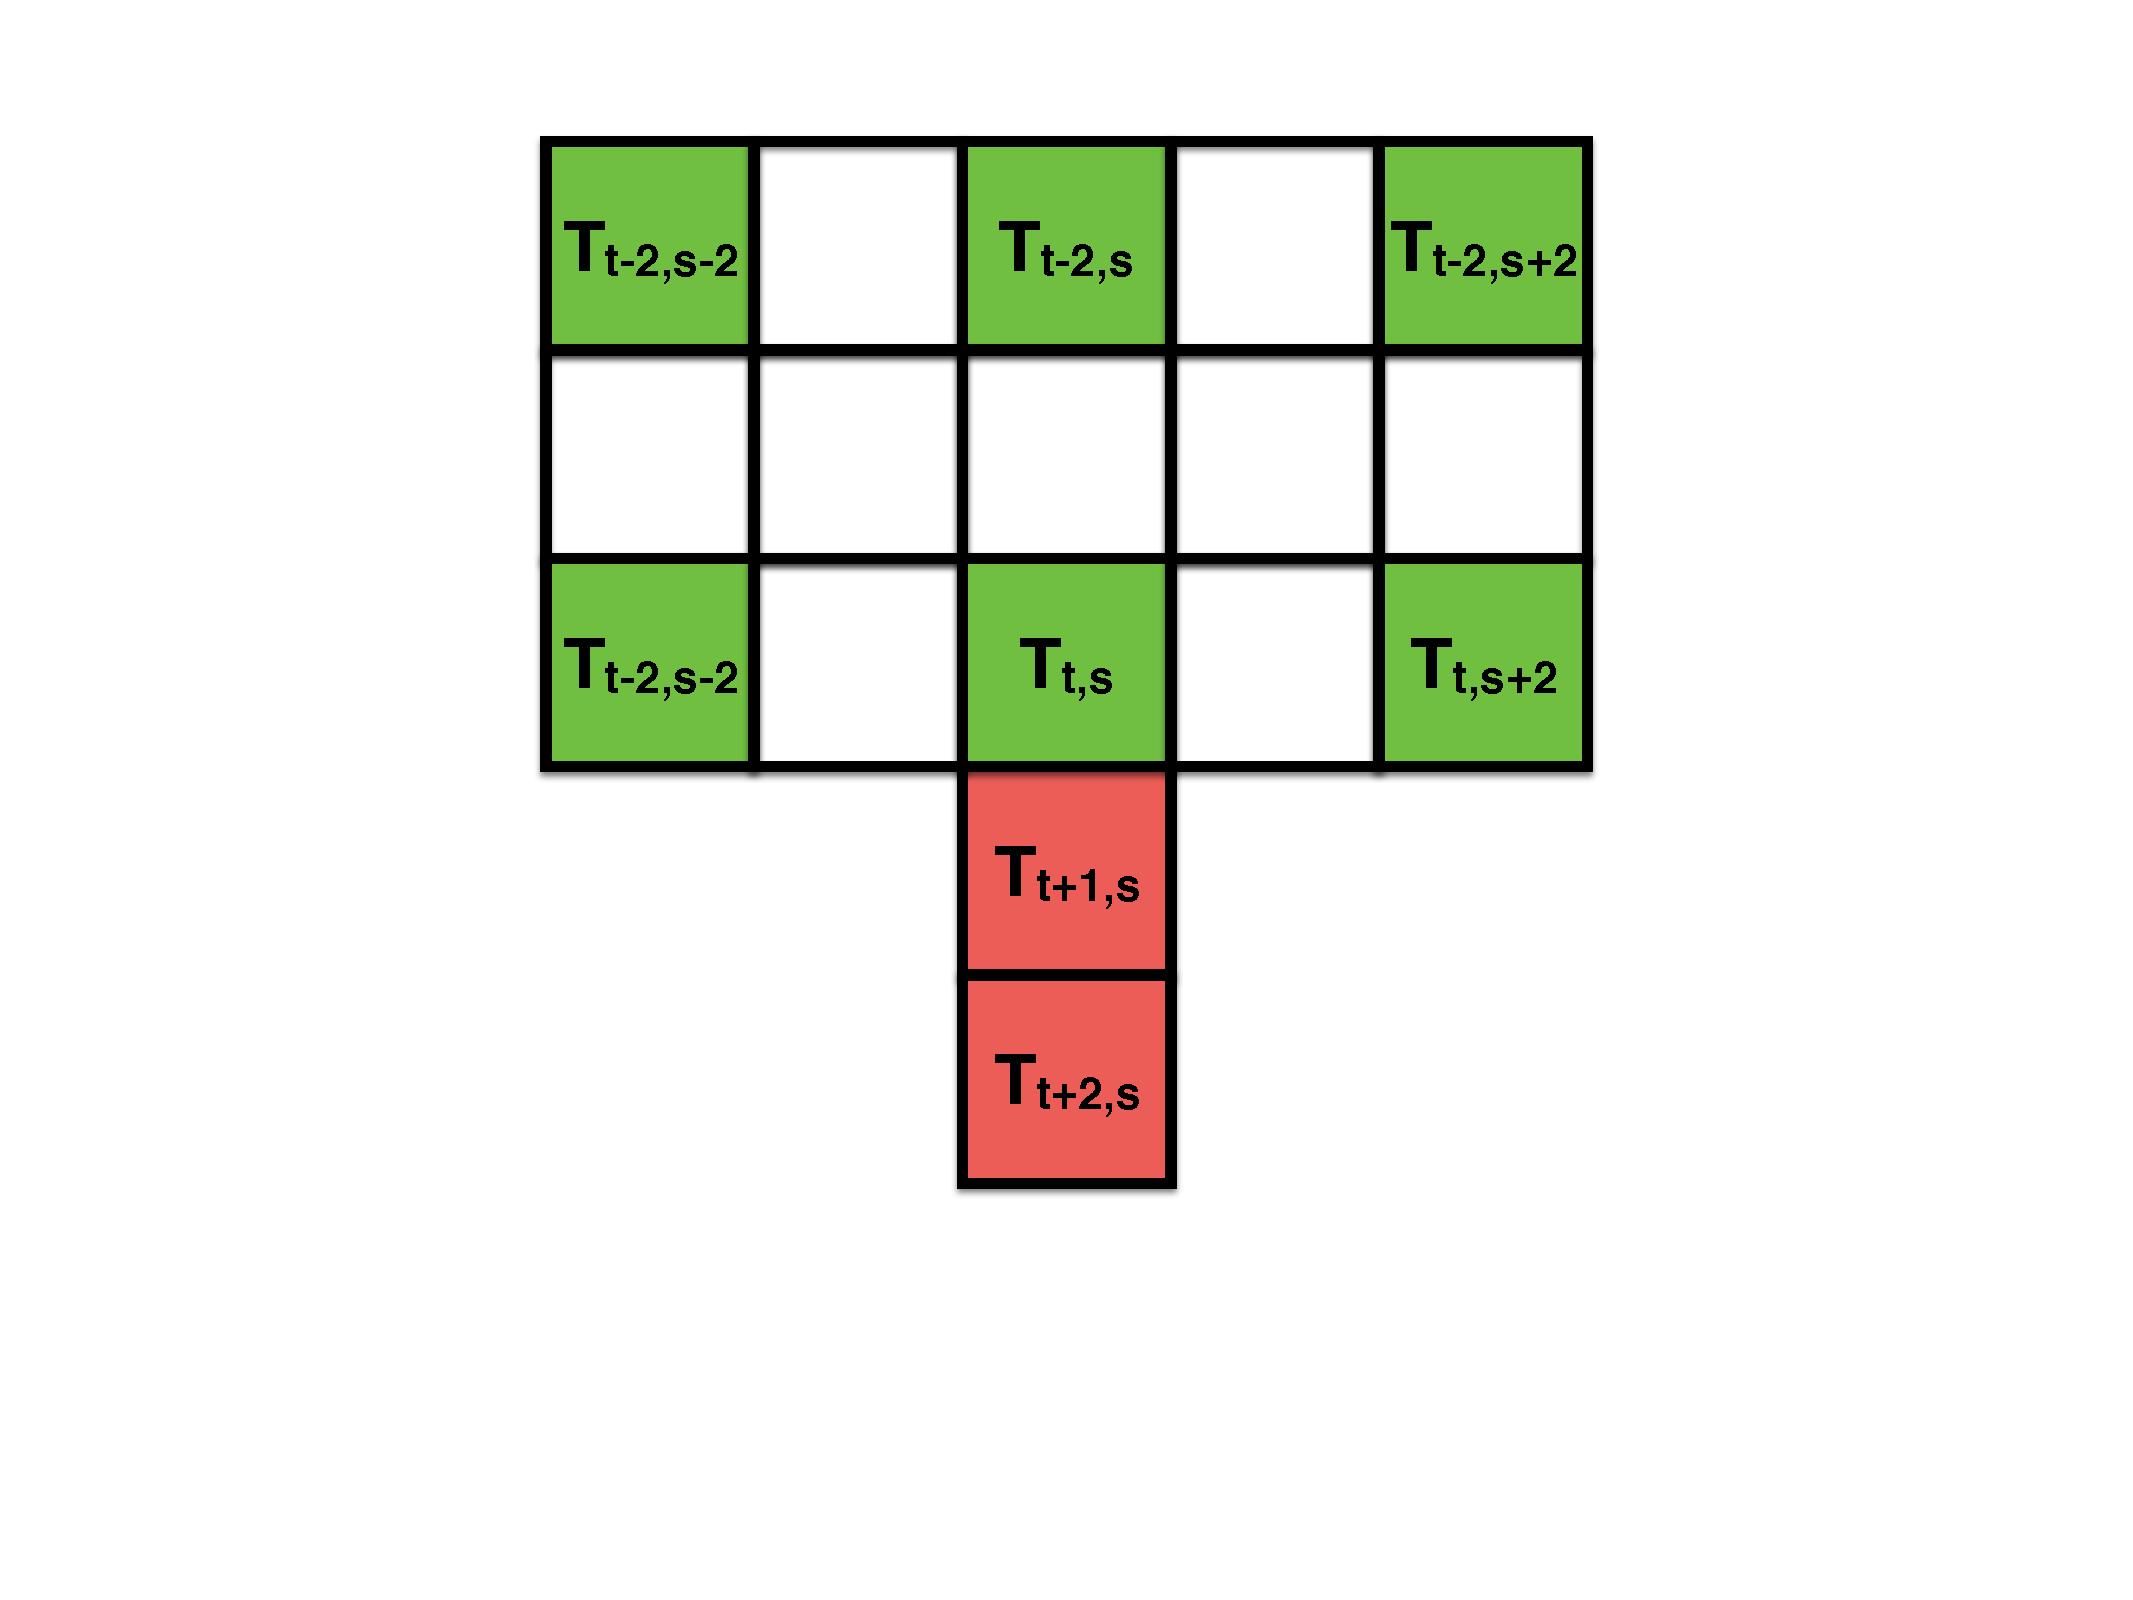
\includegraphics[width=3in]{code/2d_reshape.pdf} 
%    \caption{Embedding technique illustrating an embedding dimension of six with lag value of two in both space and time. Green is the embedded spatio-temporal series values and red is the forecast y values.}
%    \label{raw_data}
% \end{figure}



% An implementation in python is given by:

% \newpage
% \lstinputlisting[language=Python]{code_samples/ft_reshape.py}

% \newpage
% \lstinputlisting[language=Python]{code_samples/spatial_mutual_info.py}

% Additionally, splitting the space into a training set and a test set before makes the process easier. The two dimensional splitting function is represented as:

% \newpage
% \lstinputlisting[language=Python]{code_samples/2d_split.py}

% The whole two-dimensional regression technique is then wrapped into one function as:

% \newpage
% \lstinputlisting[language=Python]{code_samples/train_predict_2d.py}


% %=====================================================[Two-Dimensional Classification]
% \subsection{TWO-DIMENSIONAL CLASSIFICATION}


% The two dimensional classification is the same as the two-dimensional regression except for the classification algorithm which is represented as:

% \newpage
% \lstinputlisting[language=Python]{code_samples/nnclassification.py}

% Also the scoring function


% \newpage
% \lstinputlisting[language=Python]{code_samples/class_compare.py}


% \newpage
% \lstinputlisting[language=Python]{code_samples/full_usage.py}






% % \[x_{pred}(X_{c})=
% % \begin{cases} 
% %     1 &  \text{if } max(X_1,X_2,\dots,X_c) = X_1 \\
% %     2 &  \text{if } max(X_1,X_2,\dots,X_c) = X_2 \\
% %     \vdots \\
% %     c &  \text{if } max(X_1,X_2,\dots,X_c) = X_c
% %  \end{cases}
% % \]



% % \[F(x_t)=
% % \begin{cases} 
% %     1 &  \text{if } x_{t} = x_{pred} \\
% %     0 &  \text{if } x_{t} \neq x_{pred}
% %  \end{cases}
% % \]


% \clearpage
% %=====================================================[knn-classification]
% \subsection{Classification Example}
% The  In this section we will observe it classifying samples into one of five possible classes. Below, some test data was generated and can be seen in Figure \ref{raw_data}. This data has two features $(x_{d1},x_{d2})$, contains 100 samples, and has one target variable, $y_{d1}$, that can be one of five classes. 

% The first thing to do with this test data is the split it into a training set and a test set. We then calculate the distance between each test sample and each of the training samples. For each of the test samples, a weighted mode of the $k$ closest samples in the test set is taken. It turns out that for different numbers of $k$, we obtain different numbers of correctly classified points. This can be seen in Figure \ref{changing_k_plot}.

% One way to visualize why the percent of correctly identified points change is by this is by drawing a decision boundary as seen in Figure \ref{changing_k}. Each color in the plot corresponds to any point in that region being classified as that class. We can see that most of the points have been classified correctly, but as we increase $k$ the regions change shape. While for this example, it is slightly trivial, we will see the importance of near neighbor behavior in later examples.


% \begin{figure}[htbp] %  figure placement: here, top, bottom, or page
%    \centering
%    \includegraphics[height=3in]{code/raw_data.pdf} 
%    \caption{Example data.}
%    \label{raw_data}
% \end{figure}

% \begin{figure}[htbp] %  figure placement: here, top, bottom, or page
%    \centering
%    \includegraphics[height=3in]{code/decision_boundary.pdf} 
%    \caption{Example data with a boundary drawn in. K=5.}
%    \label{decision_boundary}
% \end{figure}


% \begin{figure}[htbp] %  figure placement: here, top, bottom, or page
%    \centering
%    \includegraphics[height=3in]{code/changing_k.pdf} 
%    \caption{Changing decision boundary based on the number of near neighbors.}
%    \label{changing_k}
% \end{figure}

% \begin{figure}[htbp] %  figure placement: here, top, bottom, or page
%    \centering
%    \includegraphics[height=3in]{code/changing_k_plot.pdf} 
%    \caption{Changing percent correct based on the number of near neighbors.}
%    \label{changing_k_plot}
% \end{figure}


% \clearpage
% %=====================================================[knn-regression]
% \subsection{Regression}
% In this section, we will explore the $k$-nearest neighbor algorithm for regression. Following the same logic above, we find the points that are closest to the point in question and calculate the mean. Likewise, it is best illustrated with an example. An example of using KNN for regression can be seen in Figure \ref{data_regression}. For this example we have generated some test points using a sine wave with a little bit of noise added on top. We will then take two-thirds of this data and use it as our training set. We will then make predictions based on the closest number of points. Again, we will be using the euclidean distance.

% After running the algorithm for different number of near neighbors, we see behavior like that shown in \ref{multiple_subplots_regression}. As we can see from the plots, as you increase the number of near neighbors, the behavior of the predictions becomes more subtle and is not a badly overfit.

% As is seen in Figure \ref{changing_k_regression}, the amount of near neighbors has about a $0.15$ difference in the $R^2$ value where $R^2$ is calculated as,



% In this expression, $y_i$ is the actual value, $f_i$ is the predicted value, and $\bar y$ is the mean of the actual values. Interestingly, we see the behavior that as we increase the number of near neighbors, our predictions get better and better. We will see this behavior again in the later sections.

% \begin{figure}[htbp] %  figure placement: here, top, bottom, or page
%    \centering
%    \includegraphics[height=3in]{code/data_regression.pdf} 
%    \caption{Data was generated using a sine wave with a little bit of noise added.}
%    \label{data_regression}
% \end{figure}


% \begin{figure}[htbp] %  figure placement: here, top, bottom, or page
%    \centering
%    \includegraphics[height=3in]{code/multiple_k_subplots.pdf} 
%    \caption{Results of predicting on one third of the data. Title is the amount of near neighbors used.}
%    \label{multiple_subplots_regression}
% \end{figure}


% \begin{figure}[htbp] %  figure placement: here, top, bottom, or page
%    \centering
%    \includegraphics[height=3in]{code/changing_k_regression} 
%    \caption{$R^2$ for prediction on one third of the data.}
%    \label{changing_k_regression}
% \end{figure}

% \subsection{Summary}
% So we have seen two ways that the K-nearest neighbor algorithm works--one classification example and one regression example. In these two examples, we only had one or two features with a single target. This algorithm will use the same fundamental principles, but b